\documentclass[12pt]{article}
\usepackage[utf8]{inputenc}
\usepackage[T1]{fontenc}
\usepackage[french]{babel}


\begin{document}

\title{Rendu 1 Projet Technologique L3}
\author{Théo Dupont}
\maketitle


\bigskip

Voici les fonctions implémentées des TP du premier semestre.\\
\\
Tous les tests sont déroulés sur 5 images différentes toutes implémentées dans l'application,
qui est elle même testée avec mon téléphone personnel, un Huawei Matte 10 Pro, sous version 9.1(Pie).
Les temps de test donnés seront sur la photo "Eye", hormis pour l'extension de dynamique en couleur, 
qui sera effectuée sur la photo "Red Gradient", et pour les convolutions qui seront réalisés sur "Sun".\\
\\
\\



L'application peut afficher 5 photos différentes en appuyant sur les 5 boutons: Eye, Mario ,Sun , Circle ,et Red Gradient respectivement.\\
L'application affichera automatiquement la hauteur et la largeur de l'image.\\
Le bouton reset permet d'afficher l'image de base sélectionnée auparavant.\\
\\
Le bouton To Gray RS applique la version de To Gray en mode RenderScript.\\
Le bouton To Grays applique quand à lui la seconde version de To Gray (avec getPixels).\\
\\
La fonction Colorize(2.1) convertit l'image en HSV pour modifier la teinte aléatoirement, puis repasser l'image en RGB.\\
Keep color (2.2) retient aléatoirement 60 degrés du cercle HSV, et passe le reste en gris. On ne choisit pas l'arc que l'on veut garder, cependant l'image Circle permet de bien mettre en avant cette fonctionnalité\\
\\
L'extension linéaire de dynamique en gris (3.1.1) augmente le contraste a partir de l'algorithme du cours.\\
Puis en couleur qui réalise la même chose sur les 3 canaux RGB(3.1.3).\\
J'ai également crée une extension linéaire de dynamique sur un seul canal, car elle serait surement plus efficace, mais cette version ne fonctionne pas. Elle est cependant disponible dans le code.\\
L'égalisation d'histograme en gris (3.2.1) aplanit l'histograme avec un autre algorithme vu en cours.\\
puis en couleur (3.2.2).\\
Il existe également deux fonctions de convolution. Une de Gauss, qui possède un masque de taille 5x5 qui applique un flou de Gauss comme prévu
L'autre effet est le moyenneur, ou l'on peut créer un masque carré de taille variable (de base 7x7) et qui applique un flou moyenneur. Sa taille peut être modifiée a souhait.
On ne modifie pas les bords des images car elles sont sufisament grandes.
\\
Toutes ces fonctions sont bien implémentées et fonctionnent correctement.
\\
Cependant, la fonction de diminution de contraste ne remplit pas son objectif. Le code de cette fonction est tout de même disponible dans le code (3.1.2)\\
\\
Il n'y a ici pas de fonctions renderScript hormis celle donnée en cours pour manque de compréhension et d'exemples de manipulations\\
\\
\\
\\
Résultats:\\
\\
Tailles images:\\
Eye: 1088*1061\\
Red Gradient: 1530*1530\\
\\
\begin{tabular}{| c | c | c |}
    \hline
    Image & Fonction & Temps (en secondes)\\ \hline
    Eye & To Grays & 1.026 \\ \hline
    Eye & To Gray RS & 0.636 \\ \hline
    Eye & Colorize & 0.837 \\ \hline
    Eye & Keep Color & 0.717 \\ \hline
    Eye & Extend Dynamic & 1.045 \\ \hline
    Red Gradient & Extend Dynamic Color & 0.824 \\ \hline
    Eye & Equalizer Gray & 0.805 \\ \hline
    Eye & Equalizer Color & 1.032 \\ \hline
    Sun & Convolution Normalizer(7x7) & 71.841 (env 2.2 sans profiler) \\ \hline
    Sun & Convolution Gauss(5x5) & 37.879 (env 1.5 sans profiler) \\ \hline
\end{tabular}
\\
\\
Exemple d'utilisation mémoire:\\
\\
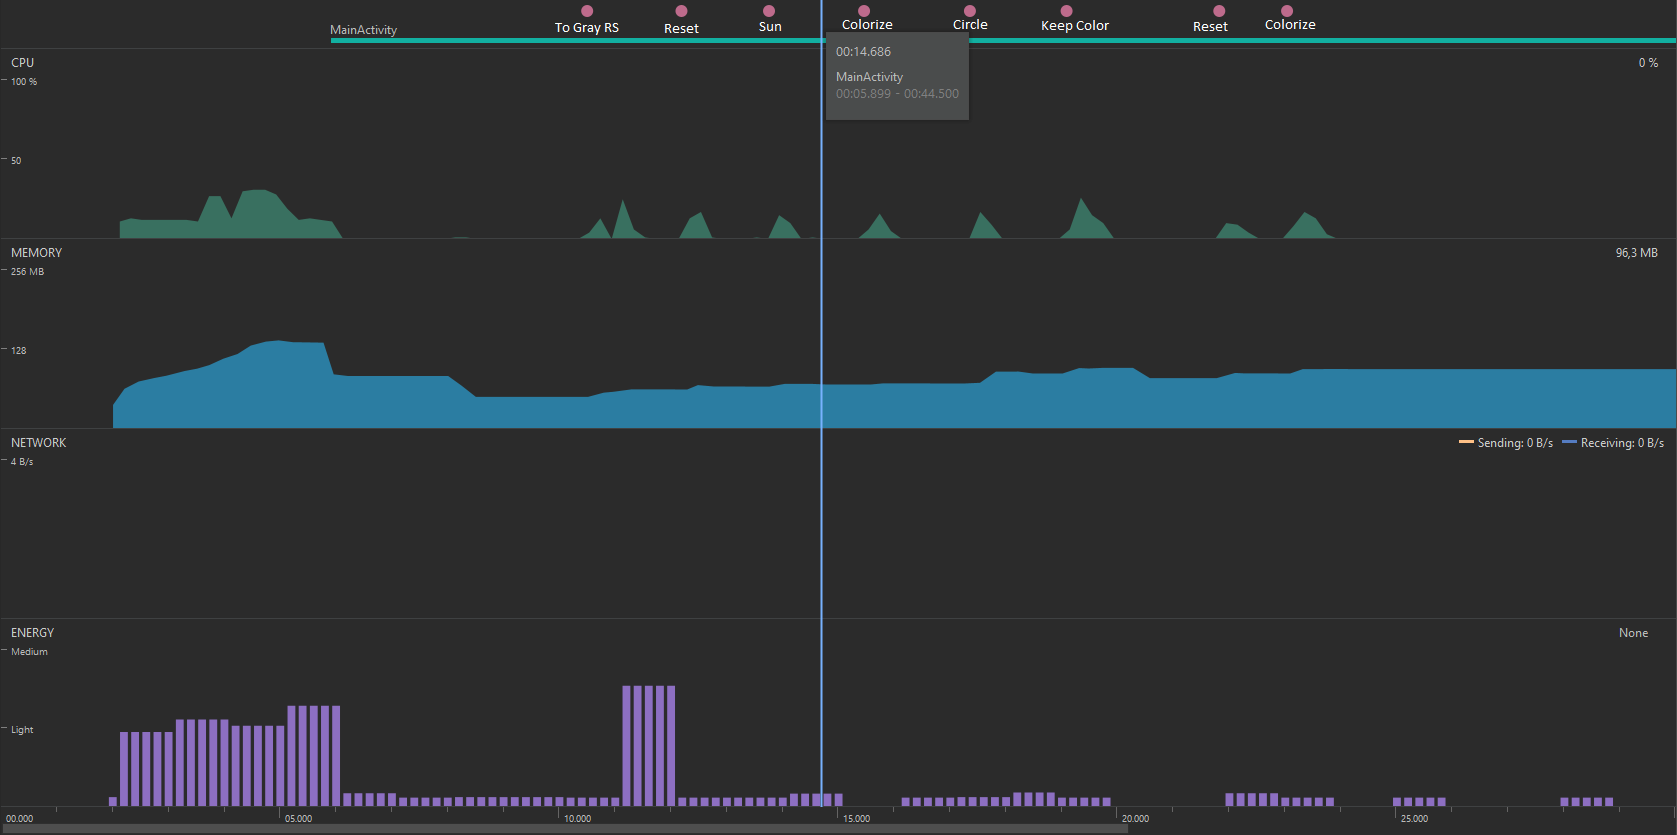
\includegraphics{./ProfilerImg.PNG}

\end{document}